%==============================================================================
% presentation.tex
%==============================================================================


%==============================================================================
% Configuration
%==============================================================================

% Internationalisation
\usepackage[utf8]{inputenc}
\usepackage[T1]{fontenc}
% \usepackage[ngerman]{babel}

% Different packages
\usepackage{url}
\usepackage{color,listings,paralist}
\usepackage{enumerate}
\usepackage{tabularx}

% Use default Acrobat reader fonts
\usepackage{mathpazo}

% Use CM fonts (increases document size)
\usepackage{ae}

% Use images
\usepackage{graphicx}

% Configure beamer
\usetheme[secheader]{Ikhono}
\usefonttheme[onlylarge]{structurebold}
\setbeamertemplate{navigation symbols}{}

% Variables
\providecommand{\Title}{Mining Software Repositories for Intelligent
  Software Maintenance}
\providecommand{\ShortTitle}{Mining software repositories}
\providecommand{\Author}{Thomas Weibel <weibelt@ethz.ch>}
\providecommand{\Institute}{SETLabs, Infosys Tech. Ltd., Bangalore}
\providecommand{\Date}{December 1, 2009}

% PDF settings
\hypersetup{
  pdftitle={\Title},
  pdfauthor={\Author},
  pdfsubject={\Institute},
  pdfkeywords={software engineering, portable, efficient, parallel
    programming language} 
}

% Titlepage
\title[\ShortTitle]{\Title}
\author{\Author}
\institute{\Institute}
\date{\Date}


%==============================================================================
% Document
%==============================================================================

\begin{document}


% Titlepage
\begin{frame}[plain]
  \titlepage
\end{frame}

\note{
  \begin{itemize}
  \item Hi and welcome to my presentation.
  \end{itemize}
}


\section{Introduction}

\begin{frame}{Executive Summary}
  \begin{itemize}
  \item TODO
  \end{itemize}
\end{frame}

\note{
  \begin{itemize}
  \item TODO
  \end{itemize}
}


\section{Framework}

\begin{frame}{Outline}
  \tableofcontents[current]
\end{frame}

\note{
  Let's have a look at our framework
}


\section{Applications}

\begin{frame}{Outline}
  \tableofcontents[current]
\end{frame}

\note{
  In this part I will show you some applications of version history mining.
}


\section{Novelty}

\begin{frame}{Outline}
  \tableofcontents[current]
\end{frame}

\note{
  Novelty of our approach.
}


\section*{Outro}

\begin{frame}{References}
  \begin{thebibliography}{10}
  % Articles
    \beamertemplatearticlebibitems
    
  \bibitem{zpl}
    B. Chamberlain et al., {\em ZPL: A Machine Independent Language
      for Parallel Computers},
    \url{http://www.cs.washington.edu/research/zpl/papers/data/Chamberlain00ZPL.pdf}
  \end{thebibliography}
\end{frame}

\note{
  Those are the are the references I used in my presentation.
}

\begin{frame}{Discussion}
  \vspace{\stretch{1}}

  \begin{center}
    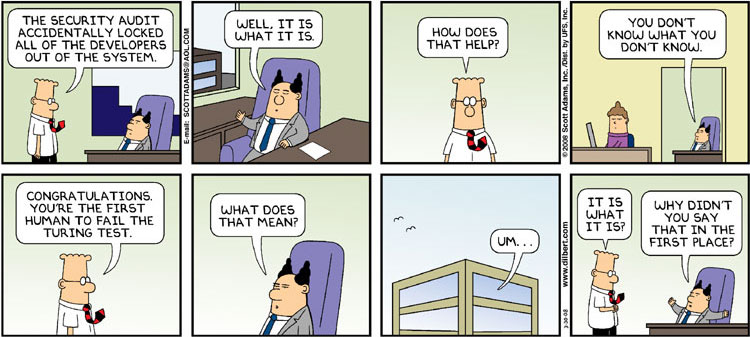
\includegraphics[width=\textwidth]{figures/dilbert-turing-test}
  \end{center}

  \vspace{\stretch{1}}
\end{frame}

\note{
}

\end{document}
